%% Direttive TeXworks:
% !TeX root = ./maltoni_niccolo_tesi.tex
% !TEX encoding = UTF-8 Unicode
% !TEX program = arara
% !TEX TS-program = arara
% !TeX spellcheck = it-IT

% arara: pdflatex: { shell: yes, synctex: yes, action: batchmode, options: "-halt-on-error -file-line-error-style" }
% arara: frontespizio
% arara: biber
% arara: pdflatex: { shell: yes, synctex: yes, action: batchmode, options: "-halt-on-error -file-line-error-style" }
% arara: pdflatex: { shell: yes, synctex: yes, action: nonstopmode, options: "-halt-on-error -file-line-error-style" }

% \begin{filecontents*}{\jobname.xmpdata}
% \Title{Progettazione object oriented di un’interfaccia grafica JavaFX per il simulatore Alchemist}
% \Author{Niccolò Maltoni}
% \Keywords{Simulazione\sep JavaFX\sep Interfaccia grafica}
% \Publisher{Università di Bologna}
% \Copyright{Copyright \copyright\ 2017 ``Niccolò Maltoni''}
% \Subject{Lo scopo di questa tesi è la progettazione di un’interfaccia grafica 2D per il simulatore Alchemist. La nuova interfaccia permette di interagire con la simulazione a tempo di esecuzione e di vedere chiaramente rappresentate informazioni su di essa; in particolare, è supportata una struttura modulare di effetti che rende facilmente osservabili determinate entità del sistema ed eventuali loro proprietà. Si è scelto di mantenere un'interfaccia il più possibile user-friendly, mantenendo un design più simile ai simulatori a scopo videoludico per favorire l'utilizzo da parte di utenti inesperti. La libreria grafica utilizzata per l'implementazione è stata JavaFX.}
% \end{filecontents*}

\documentclass[%
    a4paper,            % specifica il formato A4 (default: letter)
    12pt,               % specifica la dimensione del carattere a 12
    % openright,        % serve per aprire i capitoli sulla destra
    openany,            % serve per aprire i capitoli su qualunque pagina
    % oneside,          % serve per impaginare per stampa solo fronte
    twoside,            % serve per impaginare per stampa fronteretro
    % draft,            % evidenzia i punti in cui il testo sborda
    titlepage           % opzione necessaria per il pacchetto frontespizio
]{book}
% \usepackage[a-1b]{pdfx}
\usepackage{a4wide}             % consente di avere più spazio nell'A4

%% ORDINE IMPORTANTE INIZIO %%%%%%%%%%%%
\usepackage[T1]{fontenc}        % serve per impostare la codifica di output del font
\usepackage{textcomp}           % serve per fornire supporto ai Text Companion fonts
\usepackage[utf8]{inputenc}     % serve per impostare la codifica di input del font
\usepackage[
    english,            % utilizza l'inglese come lingua secondaria
    italian             % utlizza l'italiano come lingua primaria
]{%
    babel,                      % serve per scrivere Indice, Capitolo, etc in Italiano
    varioref                    % introduce il comando \vref da usarsi nello stesso modo del comune \ref per i riferimenti
}
\usepackage{lmodern}            % carica una variante Latin Modern prodotto dal GUST
%% ORDINE IMPORTANTE FINE %%%%%%%%%%%%%%

\usepackage{indentfirst}        % serve per avere l'indentazione nel primo paragrafo
\usepackage{setspace}           % serve a fornire comandi di interlinea standard
\usepackage{fancyhdr}           % serve per impaginare bene la tesi
\usepackage{xcolor}             % serve per la gestione dei colori nel testo
\usepackage{graphicx}           % serve per includere immagini e grafici
\usepackage{subfigure}          % serve a creare sottofigure
\usepackage{wrapfig}            % serve per includere figure "wrapped" nel testo
\usepackage[%
    write,              % alternativa a nowrite, crea il file *-frn.tex
    %nowrite,           % alternativa a write, non crea il file *-frn.tex
    standard,           % alternativa a suftesi, crea un frontespizio standard
    %signatures,        % lascia fra i nomi dei relatori lo spazio per le loro firme
    %noadvisor,         % opzione per non mostrare il relatore
    swapnames,          % scambia la posizione dei nomi di relatori e candidato
    normal              % alternativa a sans, utilizza un font "normale"
    %sans,              % alternativa a normal, utilizza un font senza grazie
    %norules,           % eliminano i filetti fra il nome dell’ateneo e quello della facoltà e sopra l’indicazione dell’anno accademico
    %nouppercase,       % disabilita il maiuscoletto nel nome della facoltà
    %noinputenc,        % disabilita la trascrizione dell'inputenc nel preambolo
    %onlyinclude        % disabilita tutte le altre opzioni
]{frontespizio}                 % serve a costruire un buon frontespizio
\usepackage[%
    strict,             % rende tutti gli warning degli errori
    autostyle,          % imposta lo stile in base al linguaggio specificato in babel
    english=american,   % imposta lo stile per l'inglese
    italian=guillemets  % imposta lo stile per l'italiano
]{csquotes}                     % serve a impostare lo stile delle virgolette
\usepackage[%
    maxcitenames=2,     % massimo numero di nomi nelle citazioni
    mincitenames=2,     % minimo numero di nomi nelle citazioni
    maxbibnames=99,     % massimo numero di nomi nella blibliografia
    minbibnames=99,     % minimo numero di nomi nella blibliografia
    style=numeric,      %
    giveninits=true,    %
    backend=biber       % specifica il backend per la bibliografia
]{biblatex}                     % si interfaccia con bibtex e biber per la bibliografia
\addbibresource{biblio.bib}
\usepackage[%
    %notbib,            % rimuove la bibliografia dall'indice
    notindex,           % rimuove l'indice dall'indice
    nottoc,             % rimuove la Table of Contents dall'indice
    notlot,             % rimuove la lista delle tabelle dall'indice
    notlof,             % rimuove la lista delle figure dall'indice
    %chapter,           % "Use chapter-level headings, if possible"
    %section,           % "Use section-level headings, if possible"
    %numbib             % numera il capitolo della bibliografia
    %numindex           % numera il capitolo dell'indice
]{tocbibind}                    % aggiunge cose all'indice
%\usepackage{fncychap}          % serve a personalizzare il formato dei titoli dei capitoli
%\usepackage[]{titlesec}        % una volta definito lo stile nel preambolo con \titleformat formatta i \chapter{}
%\usepackage{enumitem}          % serve a personalizzare liste enumerate, itemize e description
%\usepackage{amssymb}           % abilita i font matematici forniti dall’American Mathematical Society, carica anche {amsfonts}
%\usepackage{mathtools}         % carica {amsmath} e fornisce estensioni per il miglioramento della struttura informativa e della stampa di formule matematiche
%\usepackage{relsize}           % consente di assegnare dimensioni relative con i comandi \smaller e \larger

\onehalfspacing                 % Imposta interlinea a 1,5 ed equivale a \linespread{1,5}

%% TODO capire e poi decidere se inserire o no
%% produce un buon layout con fancyhdr %%%%%%%%%%%%%%%%%%%%%%%%%%%%%%%%%%%%%%
%\pagestyle{fancy}\addtolength{\headwidth}{20pt}
%\renewcommand{\chaptermark}[1]{\markboth{\thechapter.\ #1}{}}
%\renewcommand{\sectionmark}[1]{\markright{\thesection \ #1}{}}
%\cfoot{}
%
%\rhead[\fancyplain{}{\bfseries\leftmark}]{\fancyplain{}{\bfseries\thepage}}
%\lhead[\fancyplain{}{\bfseries\thepage}]{\fancyplain{}{\bfseries\rightmark}}

%% Definisce l'environment abstract per la classe book
\newenvironment{abstract}%
    {\cleardoublepage%
        \thispagestyle{empty}%
        \null \vfill\begin{center}%
            \bfseries \phantomsection%
            \addcontentsline{toc}{chapter}{\abstractname}%
            \abstractname \end{center}}%
    {\vfill\null}

% Definisco un nuovo comando per enfatizzare il testo in inglese
\newcommand{\engEmph}[1] {\emph{\foreignlanguage{english}#1}}

\usepackage[htt]{hyphenat}      % Enable hyphenation of TT text
\hyphenation{                   % Permette di sillabare bene le parole
    JavaFX
    Swing
    Micro-systems
    Script
    script
    Pack-age
    pack-age
    Manage-ment
    manage-ment
    Com-munity
    com-munity
}

\setcounter{secnumdepth}{2}     % Numera fino alla sottosezione nel corpo del testo
\setcounter{tocdepth}{3}        % Numera fino alla sotto-sottosezione nell'indice

\usepackage{hyperref}
\hypersetup{%
    pdfpagemode={UseOutlines},
    hidelinks,          % nasconde i collegamenti (non vengono quadrettati)
    linktoc=all         % inserisce i link nell'indice
    bookmarks=true,
    bookmarksopen,
    pdfstartview={FitH},
    pdfauthor={Niccolò Maltoni},
    pdftitle={Progettazione object oriented di un’interfaccia grafica JavaFX per il simulatore Alchemist}
}
\usepackage[all]{hypcap}        % sistema i problemi di hyperref

% cleveref va anche dopo hyperref
\usepackage[%
    english,italian,    % definizione delle lingue da usare
    nameinlink          % inserisce i link nei riferimenti
]{cleveref}                     % permette di usare riferimenti migliori dei \ref e dei varioref

\begin{document}
    \frontmatter
    \pagenumbering{Roman}
    %% Direttive TeXworks:
% !TeX root = ../../maltoni_niccolo_tesi.tex
% !TEX encoding = UTF-8 Unicode
% !TEX program = arara
% !TEX TS-program = arara
% !TeX spellcheck = it-IT

\begin{frontespizio}
    \Universita{Bologna}
    \Istituzione{%
        Alma Mater Studiorum - Università di Bologna \\%
        Campus di Cesena%
    }
    \Divisione{Scuola di Scienze}
    \Corso[Laurea]{Ingegneria e Scienze Informatiche}
    \Annoaccademico{2016-2017}
    \Titolo{%
        Progettazione object oriented \\%
        di un’interfaccia grafica JavaFX \\%
        per il simulatore Alchemist%
    }
    \Sottotitolo{Tesi in Programmazione ad Oggetti}
    \Candidato{Niccolò~Maltoni}
    \NCandidato{Presentata da}
    \Relatore{Prof.~Mirko~Viroli}
    \Correlatore{Ing.~Danilo~Pianini}
    \Piede{%
        II sessione di laurea \\%
        Anno Accademico 2016 - 2017%
    }
\end{frontespizio}

    %% Direttive TeXworks:
% !TeX root = ../../maltoni_niccolo_tesi.tex
% !TEX encoding = UTF-8 Unicode
% !TEX program = arara
% !TEX TS-program = arara
% !TeX spellcheck = it-IT

\clearemptydoublepage
\thispagestyle{empty}
\vspace*{20ex}
\begin{flushright}
    \begin{LARGE}
        \textbf{Parole chiave}\\
        \vspace{5ex}
    \end{LARGE}
    \begin{normalsize}
        \textbf{%
            Progettazione object-oriented\\%
            \medskip
            Simulazione\\%
            \medskip
            Java\\%
            \medskip
            JavaFX\\%
            \medskip
            Interfaccia grafica%
        }
    \end{normalsize}
\end{flushright}
\vfill

    % %% Direttive TeXworks:
% !TeX root = ../maltoni_niccolo_tesi.tex
% !TEX encoding = UTF-8 Unicode
% !TEX program = arara
% !TEX TS-program = arara
% !TeX spellcheck = it-IT

%% Direttive Arara:
% arara: pdflatex: { shell: yes, synctex: yes, action: batchmode, options: "-halt-on-error -file-line-error-style" }
% arara: frontespizio
% arara: biber
% arara: pdflatex: { shell: yes, synctex: yes, action: batchmode, options: "-halt-on-error -file-line-error-style" }
% arara: pdflatex: { shell: yes, synctex: yes, action: nonstopmode, options: "-halt-on-error -file-line-error-style" }

\null\vspace{\stretch{1}}
\begin{flushright}

    \textit{A miei genitori e in generale ad amici e parenti che mi hanno sostenuto durante questo percorso.}

\end{flushright}
\vspace{\stretch{2}}\null

    %% Direttive TeXworks:
% !TeX root = ../maltoni_niccolo_tesi.tex
% !TEX encoding = UTF-8 Unicode
% !TEX program = arara
% !TEX TS-program = arara
% !TeX spellcheck = it-IT

%% Direttive Arara:
% arara: pdflatex: { shell: yes, synctex: yes, action: batchmode, options: "-halt-on-error -file-line-error-style" }
% arara: frontespizio
% arara: bibtex
% arara: pdflatex: { shell: yes, synctex: yes, action: batchmode, options: "-halt-on-error -file-line-error-style" }
% arara: pdflatex: { shell: yes, synctex: yes, action: nonstopmode, options: "-halt-on-error -file-line-error-style" }

\begin{abstract}
    \addcontentsline{toc}{chapter}{\abstractname}
    Lo scopo di questa tesi verte intorno allo studio del simulatore Alchemist e al fine di progettare un’interfaccia 2D potenziata per l'ambiente grafico relativo alla simulazione. La nuova interfaccia permette di interagire con la simulazione a tempo di esecuzione e di vedere chiaramente rappresentate informazioni su di essa; in particolare, è supportata una struttura modulare di effetti che per rendere ancora più facilmente osservabili determinate entità del sistema ed eventuali loro proprietà. Si è scelto di mantenere un'interfaccia il più possibile \engEmph{user-friendly}, mantenendo un design più simile ai simulatori a scopo videoludico per favorire l'utilizzo da parte di utenti inesperti.

    % TODO analizza risultati

    \medskip

    La seguente trattazione è strutturata su tre capitoli: nel capitolo~\ref{ch:intro} viene introdotto il contesto nel quale il lavoro descritto nella tesi ha preso parte, introducendo il simulatore Alchemist, la sua interfaccia grafica classica e il framework JavaFX; nel capitolo~\ref{ch:contributo} si espone l'intero contributo fornito al progetto, analizzando singolarmente le fasi di analisi dei requisiti, design e progettazione e in ultimo implementazione della nuova interfaccia; infine, il capitolo~\ref{ch:conclusioni} analizza i risultati ottenuti, interpretandoli anche in ottica di miglioramenti futuri.
\end{abstract}

    \tableofcontents

    \mainmatter
    %% Direttive TeXworks:
% !TeX root = ../maltoni_niccolo_tesi.tex
% !TEX encoding = UTF-8 Unicode
% !TEX program = arara
% !TEX TS-program = arara
% !TeX spellcheck = it-IT

%% Direttive Arara:
% arara: pdflatex: { shell: yes, synctex: yes, action: batchmode, options: "-halt-on-error -file-line-error-style" }
% arara: frontespizio
% arara: biber
% arara: pdflatex: { shell: yes, synctex: yes, action: batchmode, options: "-halt-on-error -file-line-error-style" }
% arara: pdflatex: { shell: yes, synctex: yes, action: nonstopmode, options: "-halt-on-error -file-line-error-style" }

\chapter{Introduzione}\label{ch:intro}

    \section{Alchemist}\label{sec:alchemist}
        Alchemist~\cite{alchemistWeb, alchemist2013} è un meta-simulatore estendibile completamente \engEmph{open-source} che esegue su \engEmph{Java~Virtual~Machine} (JVM), nato all'interno del'Università di Bologna e distribuito su licenza GNU GPLv3+ con \engEmph{linking exception}; il codice è reperibile su GitHub\footnote{\url{https://github.com/AlchemistSimulator/Alchemist}}\label{fn:gh}, dove chiunque fosse interessato può collaborare sviluppando nuove estensioni, migliorando funzionalità esistenti e risolvendo possibili bug.

        \subsection{Introduzione ad Alchemist}\label{sub:introAlchemist}
            In generale, una \emph{simulazione}~\cite{des3} è una riproduzione del modo di operare di un sistema o un processo del mondo reale nel tempo.
            L'imitazione del processo del mondo reale è detta \emph{modello}; esso risulta essere una riproduzione più o meno semplificata del mondo reale, che viene aggiornata ad ogni passo di esecuzione della simulazione.

            Alchemist rientra nell'archetipo dei simulatori ad eventi discreti (DES)~\cite{des, des2}: gli eventi sono strettamente ordinati e vengono eseguiti uno alla volta, mentre il tempo viene fatto avanzare parallelamente ad ogni passo (detto \engEmph{tick}).
            L'idea dietro al progetto è quello di riuscire ad avere un framework di simulazione il più possibile generico, in grado di simulare sistemi di tipologia e complessità diverse, mantenendo le prestazioni dei simulatori non generici (come ad esempio quelli impiegati in ambito chimico~\cite{gillespie1976}).

            Per perseguire questo obiettivo, la progettazione dell'algoritmo è partita dallo studio del lavoro di Gillespie del 1977~\cite{gillespie1977} e di altri scienziati nell'ambito della simulazione chimica. Nonostante siano presenti algoritmi in grado di eseguire un numero di reazioni addirittura in tempo costante, la scelta dell'algoritmo è infine ricaduta su una versione migliorata dell'algoritmo SSA di Gillespie, il Next Reaction Method~\cite{nextReactionMethod} di Gibson e Bruck: ad ogni passo di simulazione, esso è in grado di selezionare la reazione successiva in tempo costante e richiede un tempo logaritmico per aggiornare le strutture dati interne al termine dell'esecuzione dell'evento.

        % \subsection{Architettura di Alchemist}\label{sub:architettura}
            % TODO analizza architettura Alchemist e separala dal modello

        \subsection{Astrazioni e modello di Alchemist}\label{sub:modello}
            Il modello di astrazione di Alchemist è ispirato dal lavoro della comunità scientifica nell'ambito dei simulatori a scopo di ricerca chimica e, dunque, ne riprende la nomenclatura, seppur con alcune libertà per favorire
            Le entità (visibile in \figurename~\vref{fig:model}) su cui lavora sono le seguenti:

            \begin{description}
                \item[\engEmph{Molecule}\label{itm:mol}]
                    Una \emph{Molecola} rappresenta il nome dato ad un particolare dato all'interno di un \emph{Nodo}, del quale ne astrae parte dello stato.

                    Un parallelismo con la programmazione imperativa vedrebbe la \emph{Molecola} come un'astrazione del nome di una variabile.

                \item[\engEmph{Concentration}\label{itm:conc}]
                    La \emph{Concentrazione} di una \emph{Molecola} è il valore associato alla proprietà rappresentata dalla \emph{Molecola}.

                    Mantenendo il parallelismo con la programmazione imperativa, la \emph{Concentrazione} rappresenterebbe il valore della variabile.

                \item[\engEmph{Node}\label{itm:node}]
                    Il \emph{Nodo} è un contenitore di \emph{Molecole} e \emph{Reazioni} che risiede all'interno di un \emph{Ambiente} e che astrae una singola entità.

                \item[\engEmph{Environment}\label{itm:env}]
                    L'\emph{Ambiente} è l'astrazione che rappresenta lo spazio nella simulazione ed è l'entità che contiene i nodi.

                    Esso è in grado di fonrire informazioni in merito alla posizione dei \emph{Nodi} nello spazio, alla distanza tra loro e al loro vicinato; opzionalmente, l'\emph{Ambiente} può offrire il supporto allo spostamento dei \emph{Nodi}.

                \item[\engEmph{Linking rule}\label{itm:linkr}]
                    La \emph{Regola di collegamento} è la funzione dello stato corrente dell'\emph{Ambiente} che associa ad ogni \emph{Nodo} un \emph{Vicinato}.

                \item[\engEmph{Vicinato}\label{itm:neigh}]
                    Un \emph{Vicinato} è un'entità costituita da un \emph{Nodo} detto ``centro'' e da un insieme di altri \emph{Nodi} (i ``vicini'').

                    L'astrazione dovrebbe avere un'accezione il più possibile generale e flessibile, in modo da poter modellare qualsiasi tipo di legame di vicinato, non solo spaziale.

                \begin{figure}[htbp]\label{fig:react}
                    \centering
                    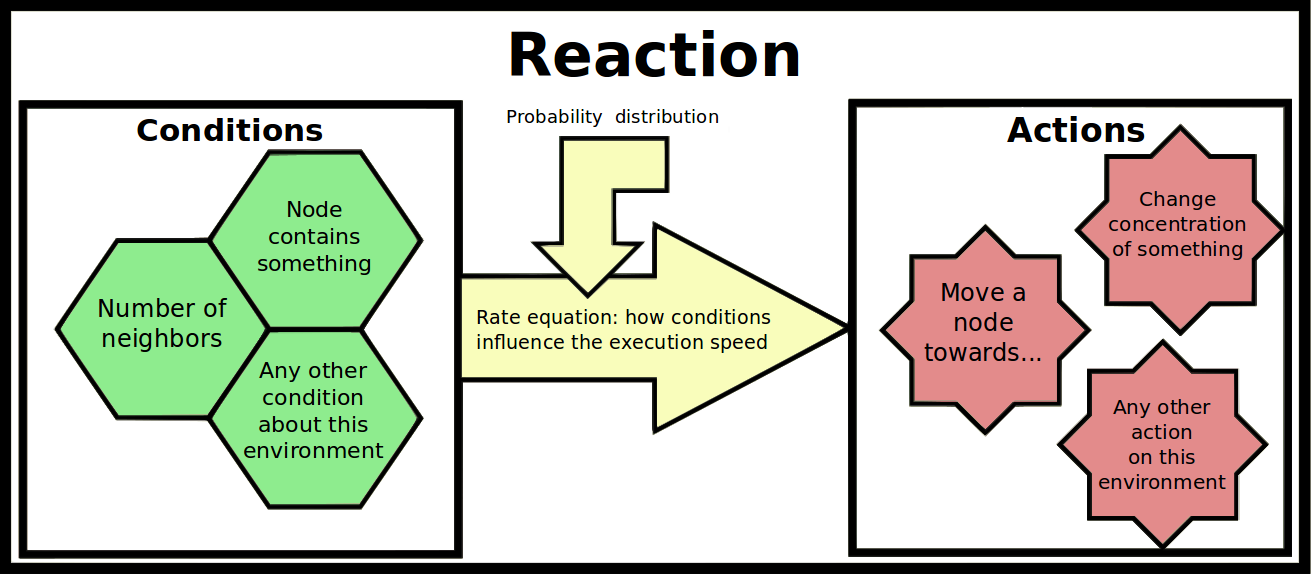
\includegraphics[scale=.35]{img/reaction}
                    \caption{%
                        La figura, rivisitata da quella disponibile sul sito ufficiale~\cite{alchemistWeb}, offre una rappresentazione grafica della \emph{Reazione}.
                    }
                \end{figure}

                \item[\engEmph{Reaction}\label{itm:react}]
                    Il concetto di \emph{Reazione} è da considerarsi molto più elaborato di quello utilizzato in chimica: in questo caso, si può considerare com un insieme di \emph{Condizioni} sullo stato del sistema, che qualora dovessero risultare vere innescherebbero l'esecuzione di un insieme di \emph{Azioni}.

                    Una \emph{Reazione} (di cui è possibile vederne una rappresentazione grafica in \figurename~\vref{fig:react}) è dunque un qualsiasi evento che può cambiare lo stato dell’\emph{Ambiente} e si compone di un insieme di condizioni, una o più azioni e una distribuzione temporale.

                    La frequenza di accadimento può dipendere da:
                    \begin{itemize}
                        \item[--] Un tasso statico;
                        \item[--] Il valore di ciascuna \emph{Condizione};
                        \item[--] Una equazione che combina il tasso statico e il valore delle \emph{Condizioni}, restituendo un ``tasso istantaneo'';
                        \item[--] Una distribuzione temporale.
                    \end{itemize}

                    Ogni \emph{Nodo} è costituito da un insieme (anche vuoto) di \emph{Reazioni}.

                \item[\engEmph{Condition}\label{itm:cond}]
                    Una \emph{Condizione} è una funzione che associa un valore numerico e un valore booleano allo stato corrente di un \emph{Ambiente}.

                \item[\engEmph{Action}\label{itm:act}]
                        Un'\emph{Azione} è una procedura che provoca una modifica allo stato dell'\emph{Ambiente}.

            \end{description}

            \begin{figure}[htbp]\label{fig:model}
                \centering
                \includegraphics[scale=.4]{img/model}
                \caption{%
                    La figura, presa dal sito ufficiale~\cite{alchemistWeb}, offre una rappresentazione grafica delle diverse entità. All’interno di un ambiente, che modella il sistema, si trovano i nodi connessi tra loro attraverso dei collegamenti; ogni nodo è composto da reazioni e molecole, ognuna delle quali ha associata una concentrazione.
                }
            \end{figure}

            % TODO aggiungi dettagli
        \subsection{Interfaccia utente classica}\label{sub:prevGui}
            L'architettura di Alchemist è progettata con paradigma \engEmph{Model-View-Controller} (MVC)~\cite{mvc}, di conseguenza la suddivisione tra componente grafica (\engEmph{View}) e il blocco ``logico'' composto da \engEmph{Model} e \engEmph{Controller} è netta.
            Questa distinzione è evidente anche per quanto riguarda l'utilizzo pratico del software: una simulazione su Alchemist può venire lanciata da terminale, senza che alcuna interfaccia grafica sia necessaria per tutta la durata del periodo di esecuzione, oppure essere inizializzata, lanciata e controllata in tempo reale dalla sua interfaccia grafica.

            Per lo scopo di questa tesi, tratteremo esclusivamente della GUI.

            \subsubsection{Esperienza utente}\label{subsub:prevUx}
                Un'interfaccia grafica (detta anche GUI, \engEmph{graphical user interface}~\cite{gui}) è l’insieme dei componenti grafici con i quali l'utente può interagire per impartire comandi ad un programma del computer, che si contrappone ad un altro metodo di interazione, l'interfaccia a riga di comando (o CLI, \engEmph{Command Line Interface}).

                L'interfaccia grafica è stata ideata negli anni `80 a partire da un'esigenza di maggiore usabilità rispetto dalla riga di comando, derivante soprattuto dall'affermarsi degli studi di usabilità~\cite{norman1988} e di ergonomia cognitiva di quel periodo.

                Più ampio e moderno è invece il concetto di esperienza utente~\cite{ux} (spesso abbreviata in UX, \engEmph{User eXperience}): l'ISO 9241-210~\cite{iso9421} al definisce come ``le percezioni e le reazioni di un utente che derivano dall’uso o dall’aspettativa d’uso di un prodotto, sistema o servizio''.
                Di fatto, essa descrive la reazione dell'utente di fronte all'interazione con il programma o lo strumento in base a tre dimensioni:
                \begin{itemize}
                    \item[--] \emph{Dimensione pragmatica}: funzionalità e usabilità del sistema;
                    \item[--] \emph{Dimensione estetica/edonistica}: piacevolezza estetica, emotiva e ludica del sistema;
                    \item[--] \emph{Dimensione simbolica}: attributi sociali, forza del brand, identificazione.
                \end{itemize}
                L'usabilità, invece, fa riferimento unicamente ai soli aspetti pragmatici (la capacità di svolgere un compito con efficienza ed efficacia).

                L'interfaccia utente classica di Alchemist è caratterizzata da un'usbilità appena sufficiente, funzionale alle necessità di un utilizzatore esperto, ma non adeguato a fornire un'esperienza completa e \engEmph{user-friendly} ad un utente ``standard''.

                Grazie a contributi recenti~\cite{casadio}, la GUI ha subito un parziale rinnovamento, limitati alla parte di ambiente integrato che accoglie l'utilizzatore che stia lanciando il simulatore senza una simulazione specificata; questa parte non è oggetto del lavoro illustrato in questa tesi. Al contrario, è interessante analizzare lo stato dell'interfaccia relativa all'ambiente di esecuzione della simulazione.

                La criticità principale, che va a minare non solo il livello di esperienza utente, ma anche il concetto di usabilità  ``classico'', è evidente nella non intuitività dei controlli: come è possibile vedere in \figurename~\vref{fig:oldMain}, non sono presenti bottoni di interazione per, ad esempio, avviare o fermare la simulazione o per cambiare la modalità di interazione con la zone in cui viene rappresentato l'environment; questo perché molte possibilità di controllo sono limitate a scorciatoie da tastiera non modificabili e non esplicate altrove se non nella documentazione.

                \begin{figure}[htbp]\label{fig:oldMain}
                    \centering
                    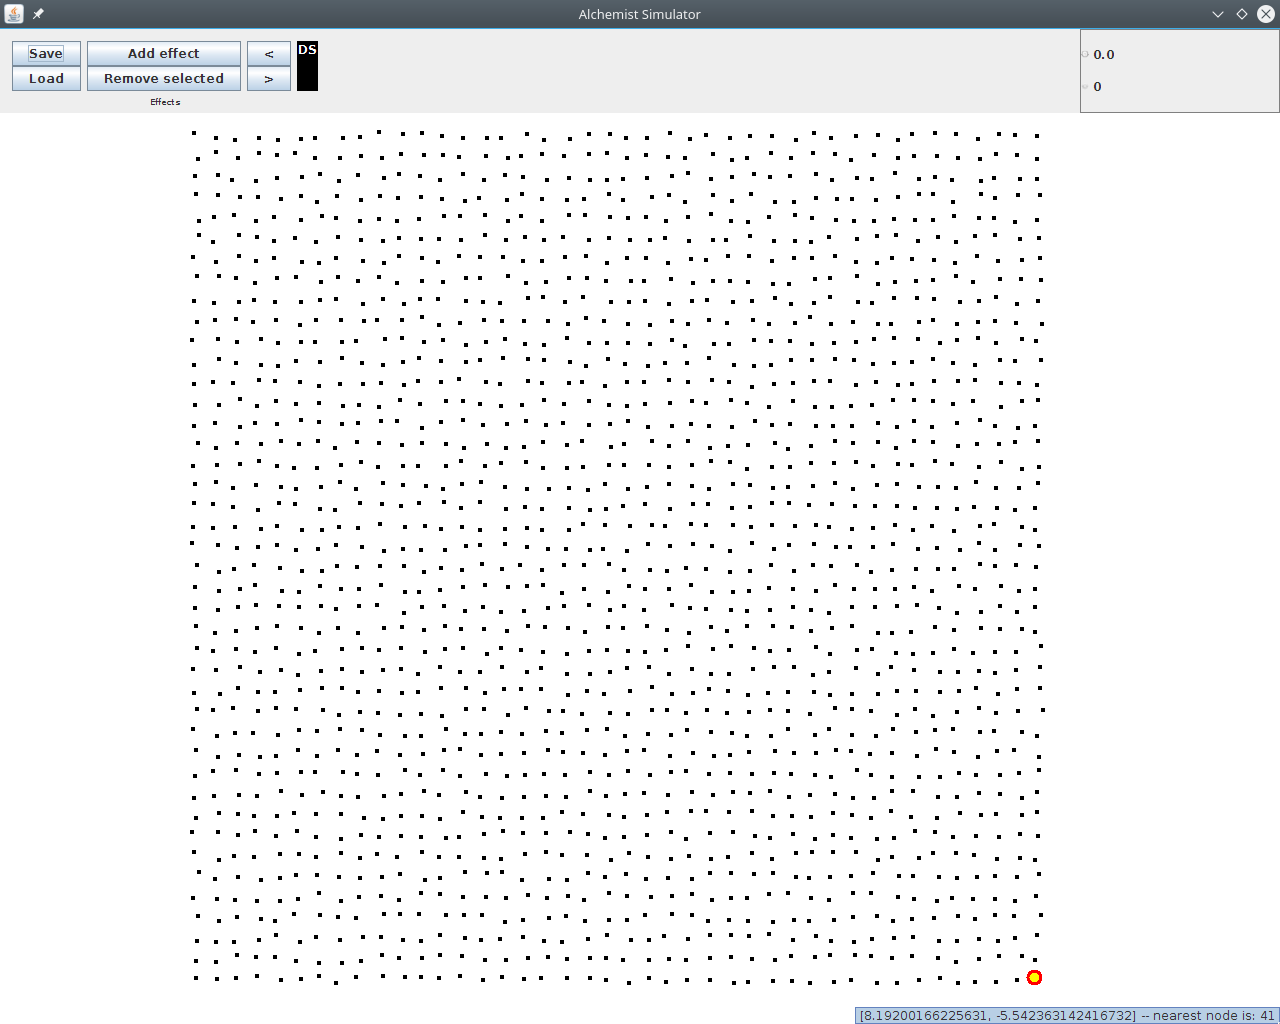
\includegraphics[scale=.35]{img/oldMain}
                    \caption{Vista principale di una simulazione con l'interfaccia classica}
                \end{figure}

                Un'ultima criticità che esula dal contesto pratico, ma che rientra appieno nel contesto estetico/edonistico importante per una buona UX è, appunto l'aspetto grafico: l'intera interfaccia di simulazione è implementata sfruttando le impostazioni di base del framework Swing, senza alcun tipo di personalizzazione estetica che rispettasse le direttive di un design grafico ben definito (come il Material Design~\cite{material} di Google o Modern UI e Fluent Design System~\cite{fluent} di Microsoft) o che mantenesse il design fornito dal sistema operativo.

            \subsubsection{Swing}\label{subsub:swing}
                Come detto, Alchemist utilizzava Swing come strumento per implementare l'interfaccia grafica. Java Swing è un framework per lo sviluppo di GUI in Java, parte delle \engEmph{Java Foundation Classes} (JFC) insieme ad AWT (\engEmph{Abstract Window Toolkit}) e \emph{Java 2D}.

                Come è possibile vedere in \figurename~\vref{fig:awt}, la libreria sfrutta i componenti forniti da AWT, mettendo a disposizione nuovi componenti in grado di risolvere diverse debolezze del precedente standard grafico per il linguaggio di Oracle:

                \begin{figure}[htbp]\label{fig:awt}
                    \centering
                    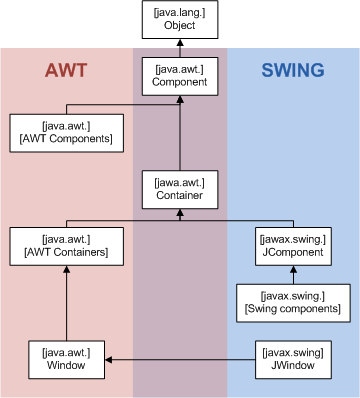
\includegraphics[scale=.45]{img/AWTSwing}
                    \caption{Struttura delle classi di Swing e AWT, by Jakub Závěrka (Jakub Závěrka - own work) [Public domain], via Wikimedia Commons}
                \end{figure}

                \begin{itemize}
                    \item[--] Swing è molto più facilmente estendibile e rende possibile un controllo della presentazione grafica dei componenti (il \engEmph{look'n'feel}) trasparente, non necessitando più di classi specifiche per ogni aspetto grafico.

                    \item[--] I componenti forniti da Swing permettono inoltre di realizzare un'interfaccia più leggera di quella di AWT: essa sfrutta infatti le API fornite da Java 2D, anziché chiamare il \engEmph{toolkit} di interfacce native del sistema operativo; nel contempo, appoggiandosi al container di AWT, sfrutta l'accesso al framework di gestione delle GUI fornito dall'OS, traducendo gli eventi specifici dell'OS in eventi Java disaccoppiati dalla piattaforma su cui gira la JVM, semplificando la gestione da parte dello sviluppatore.

                    \item[--] Swing rende più semplice appoggiarsi al pattern MVC per implementare software con GUI, separando le classi di modello da quelle grafiche e di controllo.

                \end{itemize}

            \subsubsection{Gli effetti e l'interfaccia \texttt{Effect}}\label{subsub:effect}
                Una parte consistente della visualizzazione di una simulazione di Alchemist, nell'interfaccia classica come in quella attuale, è costituita dagli effetti.

                Un \emph{effetto} in Alchemist è una rappresentazione grafica di ``qualcosa'' nell'ambiente; costituisce di fatto una modalità semplificata per l'utente di cogliere quanto accade nella simulazione.

                L'interfaccia Java che implementa questo tipo di astrazione prima del lavoro svolto con questa tesi è la classe \texttt{Effect}.
                L'effetto è in grado di rappresentare qualsiasi proprietà di un nodo dato; è concepito come un oggetto serializzabile, in modo da semplificare il salvataggio e il caricamento di intere rapprsentazioni tramite la serializzazione di collezioni di essi.

    \section{JavaFX}\label{sec:jfx}
        Nel mese di maggio del 2007 alla conferenza annuale JavaOne, Sun Microsystems annuncia JavaFX Script (chiamato anche F3, \engEmph{Form~Follows~Function}), un DSL (\engEmph{Domain~Specific~Language}, linguaggio di dominio specifico) pensato per lo sviluppo di interfacce grafiche di Rich Internet Applications~\cite{moritz2008rich}, e JavaFX Mobile, un sistema software per dispositivi mobili basato su Java e ispirato all'allora neonato iPhone, che avrebbe avuto come cavallo di battaglia la possibilità di sviluppare app mobile in grado di condividere codice e asset grafici con le controparti desktop e web, semplificando lo sviluppo di ecosistemi strutturati.

        Incluso nella versione 1.0 del pacchetto JavaFX rilasciato nel dicembre del 2008, JavaFX Script verrà però abbandonato da Oracle (che nel frattempo aveva acquisito Sun Microsystems) meno di 2 anni dopo, in contemporanea con l'ampliamento della disponibilità delle JavaFX API agli altri linguaggi disponibili per JVM; anche JavaFX Mobile, con l'avvento di OS mobili moderni come Android e iOS, può considerarsi deprecato.

        JavaFX continua invece lo sviluppo come framework per la gestione di interfacce grafiche per Java ed altri linguaggi JVM-compatibili, andando di fatto a sostituire Swing e AWT.

        In questo capitolo si intende analizzare il framework e le sue funzionalità fino alla versione utilizzata nella stesura del codice, nonché l'ultima versione stabile all'atto di inizio del lavoro illustrato in questa tesi: JavaFX 8.

        \subsection{Introduzione al framework JavaFX}\label{sub:jfxIntro}
            La prima versione di JavaFX ad abbandonare JavaFX Script e JavaFX Mobile, con i quali il framework era nato, per andare ad affiancarsi a Swing è la versione 2.0, distribuita parzialmente su licenza \engEmph{open-source} verso la fine del 2011.
            Essa introduceva un nuovo linguaggio XML dichiarativo, l'FXML, in grado di fornire una struttura grafica all'applicazione coinvolgendo minimamente il codice Java, oltre a migliorare il supporto \engEmph{multi-thread}.
            Con le successive versioni 2.1 e 2.2, rilasciate nell'arco del 2012, viene esteso il supporto a MacOS e Linux.

            La prima versione ad essere parte del JRE/JDK è JavaFX 8, rilasciata il 18 marzo 2014 insieme a Java 8; essa diventa di fatto la nuova libreria di riferimento per lo sviluppo di applicazioni grafiche per ambiente JVM.

            Essa si presenta come fortemente orientata verso i pattern di progettazione \engEmph{Model-View-Controller} e \engEmph{Model-View-Presenter}; la suddivisione infatti è netta:
            \begin{itemize}
                \item[--] La \emph{componente visiva} è definita su file di markup FXML, logicamente separati da qualsiasi componente Java che non siano le loro classi \engEmph{Controller}; anche la \emph{presentazione}, definibile attraverso fogli di stile CSS, è indipendente dalle altre componenti Java e XML e può essere anche sostituita a tempo di esecuzione senza difficoltà;
                \item[--] Il \emph{controllo} dell'applicazione è circoscritto a classi Java specifiche, che vengono associate al caricamento del documento di markup corrispondente; per design sono facilmente sostituibili da differenti implementazioni progettate per interagire con gli oggetti che il parser di JavaFX riconosce nel file FXML;
                \item[--] In una implementazione che sfrutti appieno gli strumenti messi a disposizione del framework, per design il \emph{modello} non viene coinvolto delle suddette componenti e resta dunque distaccato dalle suddette componenti.
            \end{itemize}

            Oltre al già citato miglioramento per quanto riguarda il \engEmph{look'n'feel} (che ora può vantare la semplificazione data dai fogli di stile CSS), un ulteriore flessibilità grafica è il supporto Hi-DPI, che permette alle GUI di adattarsi a qualsiasi risoulzione di schermo senza comprometterne la qualità.

        \subsection{Architettura del framework JavaFX}\label{sub:jfxFramework}
            Come è possibile osservare in \figurename~\vref{fig:jfxArch}, l'architettura interna di JavaFX è costituita da diversi livelli, ciascuno dei quali sfrutta le funzionalità messe a disposizione dai livelli inferiori per offrire nuove API ai livelli superiori e allo sviluppatore finale.

            Il livello più elevato per la costruzione di una applicazione JavaFX è il grafo delle scene (\engEmph{Scene Graph}): esso ospita un albero gerarchico di nodi, ciascuno dei quali rappresentante un elemento visivo dell'interfaccia utente. Questo livello si occupa anche di intercettare gli input e di mettere a disposizione le JavaFX API pubbliche.

            Un singolo elemento del grafo delle scene è chiamato \emph{nodo}. Ogni nodo possiede un ID, una classe di stile e un volume delimitato; fatta eccezione per il nodo radice, ogni nodo possiede un solo nodo genitore e può essere a sua volta genitore di uno o più altri nodi. Su ogni nodo possono essere definiti effetti grafici (come blur e ombre) e livello di opacità, nonché stati specifici per l'applicazione e comportamenti in caso di eventi specifici.

            Il livello subito inferiore allo \engEmph{Scene Graph} è costituito dal \engEmph{JavaFX Graphics System} (in \figurename~\ref{fig:jfxArch} è rappresentato dagli elementi in azzurro), che attraverso il \engEmph{Quantum Toolkit} e \engEmph{Prism} mette a disposizione funzionalità più a basso livello per rappresentazioni 2D e 3D.

            I processi di \engEmph{Prism} si occupano del rendering; possono eseguire sia con accelerazione hardware che senza, ed effettuano sia rendering 2D che 3D.
            Attraverso questi processi vengono eseguite le rasterizzazioni e i rendering di tutti i grafi delle scene.

            Il \engEmph{Quantum Toolkit} collega invece \engEmph{Prism} al \engEmph{Glass Windowing Toolkit} e gestisce le regole di threading per rendering e gestione degli eventi.

            \begin{figure}[htbp]\label{fig:jfxArch}
                \centering
                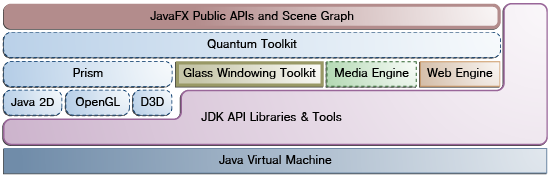
\includegraphics[scale=0.75]{img/jfxArch}
                \caption{La figura, presa dalla documentazione ufficiale di Oracle~\cite{java8}, rappresenta i diversi livelli che caratterizzano il framework JavaFX}
            \end{figure}

            Il terzo livello è costituito dal sopra citato \engEmph{Glass Windowing Toolkit}, che rappresenta il livello più basso del \engEmph{JavaFX graphics stack}.
            Esso si occupa di gestire i servizi nativi forniti dai sistemi operativi per la gestione delle finestre e delle code degli eventi; costituisce la parte \engEmph{platform-dependent} di JavaFX.

            \engEmph{Media Engine} e \engEmph{Web Engine} si occupano del supporto per i file multimediali audiovisivi e per i linguaggi web.

        \subsection{Struttura di una Applicazione JavaFX}\label{sub:jfxStruttura}

            JavaFX fornisce le classi di base per strutturare una applicazione completa, delimitando linee guida ben specifiche nella suddivisione della struttura.

            \begin{figure}[htbp]\label{fig:jfxLife}
                \centering
                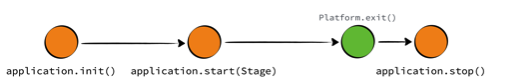
\includegraphics[scale=1]{img/jfxLifecycle}
                \caption{La figura rappresenta il ciclo di vita di una applicazione JavaFX}
            \end{figure}

            % La classe principale per una applicazione JavaFX deve estendere da \texttt{javafx\allowbreak .\allowbreak application\allowbreak .\allowbreak Application}. Il metodo \texttt{start()} è il punto di ingresso principale: lanciando una JavaFX Application attraverso il metodo \texttt{launch()} della classe di supporto \texttt{javafx\allowbreak .\allowbreak application\allowbreak .\allowbreak Platform}, verrà inizializzato il framework e poi verranno chiamati in ordine i metodi \texttt{init()} e \texttt{start(\allowbreak javafx\allowbreak .\allowbreak stage\allowbreak .\allowbreak Stage)}, che rappresentano di fatto il ciclo di inizializzazione ideale dell'applicazione.

            La classe principale per una applicazione JavaFX deve estendere da \texttt{javafx\dothyp application\dothyp Application}. Il metodo \texttt{start()} è il punto di ingresso principale: lanciando una JavaFX Application attraverso il metodo \texttt{launch()} della classe di supporto \texttt{javafx\dothyp application\dothyp Platform}, verrà inizializzato il framework e poi verranno chiamati in ordine i metodi \texttt{init()} e \texttt{start(javafx\dothyp stage\dothyp Stage)}, che rappresentano di fatto il ciclo di inizializzazione ideale dell'applicazione.
            Il metodo \texttt{main()} non deve essere necessariamente implementato perché l'applicazione possa essere avviata: esso viene infatti creato da l\engEmph{JavaFX Packager tool} durante l'inserimento del \engEmph{JavaFX Launcher} nel file JAR.

            Il layout con cui un'applicazione JavaFX è costituita a livello grafico si struttura gerarchicamente su tre sezioni principali, visibili in \figurename~\vref{fig:jfxStage}:

            \begin{description}
                \item[\texttt{Stage}] In JavaFX, una finestra è astratta tramite la classe \texttt{javafx\dothyp stage\dothyp Stage}: letteralmente ``\emph{palcoscenico}'',  è il contenitore di livello più elevato e funge da ``guscio esterno'' per ogni altro componente grafico e pannello.

                Lo \texttt{Stage} primario viene costruito dalla piattaforma all'atto di avvio, ma ulteriori \texttt{Stage} possono venire costruiti durante l'esecuzione, purché attraverso il \engEmph{JavaFX Application Thread}.

            \begin{figure}[htbp]\label{fig:jfxStage}
                \centering
                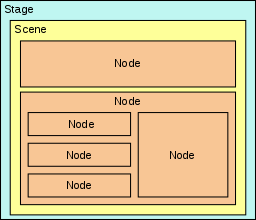
\includegraphics[scale=1]{img/Javafx-stage-scene-node}
                \caption{Struttura del layout di una applicazione JavaFX, by Stkl [CC BY-SA 4.0], via Wikimedia Commons}
            \end{figure}

                \item[\texttt{Scene}] Il contenuto dello \texttt{Stage} è rappresentato dalla classe \texttt{javafx\dothyp scene\dothyp Scene}, che è a sua volta contenitore di ogni nodo appartentente a quello specifico \engEmph{scene graph}.

                \item[\texttt{Pane}] Come già affermato nella Sezione~\vref{sub:jfxIntro}, ogni elemento appartenente ad una \emph{scena} è detto \emph{nodo}. Il terzo livello è costituito da un particolare tipo di nodo, detto \emph{pannello} (modellato dalla classe \texttt{javafx\dothyp scene\dothyp layout\dothyp Pane}), che costituisce il contenuto di una scena e gestisce la disposizione dei nodi al suo interno sullo schermo; è possibile costruire una struttura gerarchica inserendo all'interno di un pannello radice altri pannelli.
            \end{description}

            % TODO aggiungi analisi di Pannelli, Componenti e Stile

        \subsection{Vantaggi di JavaFX su Swing}\label{sub:jfxVantaggi}
    \section{Interfaccia JavaFX per Alchemist: motivazioni}\label{sec:motivi}

    %% Direttive TeXworks:
% !TeX root = ../maltoni_niccolo_tesi.tex
% !TEX encoding = UTF-8 Unicode
% !TEX program = arara
% !TEX TS-program = arara
% !TeX spellcheck = it-IT

%% Direttive Arara:
% arara: pdflatex: { shell: yes, synctex: yes, action: batchmode, options: "-halt-on-error -file-line-error-style" }
% arara: frontespizio
% arara: biber
% arara: pdflatex: { shell: yes, synctex: yes, action: batchmode, options: "-halt-on-error -file-line-error-style" }
% arara: pdflatex: { shell: yes, synctex: yes, action: nonstopmode, options: "-halt-on-error -file-line-error-style" }

\chapter{Contributo}\label{ch:contributo}
    In questo capitolo verrà analizzato il contributo fornito al progetto, elencando i requisiti necessari e analizzando il processo di soddisfazione degli stessi.

    L'obiettivo principale è quello di integrare una nuova interfaccia per la simulazione, al fine di semplificare l’adozione del simulatore da parte di utenti inesperti.

    \section{Analisi dei requisiti}\label{sec:analisi}
        Lo studio del lavoro illustrato in questa tesi ha inizio con l'analisi dei requisiti dell’interfaccia utente, ossia cosa l'applicazione deve mostrare a schermo.

        Questa sezione si occuperà di enunciare i requisiti funzionali e non funzionali individuati.

        \subsection{Requisiti funzionali}\label{sub:funzionali}
            I requisiti funzionali (\figurename~\ref{fig:useCase}) descrivono il comportamento che il sistema deve avere:
            descrivono le funzionalità del sistema software, in termini di servizi che il sistema software deve fornire, di come il sistema software reagisce a specifici tipi di input e di come si comporta in situazioni particolari.

            \subsubsection{Rappresentazione dell'ambiente di simulazione}\label{subsub:seeEnv}
                Essendo la componente grafica da reimplementare quella legata alla simulazione in escuzione, requisito fondamentale è che la GUI possa rappresentare l'ambiente con le maggiori possibilità di dettaglio possibile.

                Di conseguenza, deve essere presente uno spazio disegnabile in cui si possa avere una rappresentazione grafica di quanto accade, ma anche contatori che mostrino l'avanzamento della simulazione in termini di tempo (secondi) trascorso e passaggi (\engEmph{step}) effettuati.

            \subsubsection{Gestione degli effetti}\label{subusub:manageEffects}
                La nuova interfaccia deve rendere possibile all'utente di poter aggiungere nuovi effetti allo \engEmph{stack} di rappresentazione e modificarne le proprietà a tempo di esecuzione.

                Inoltre attraverso la GUI l'utente deve poter salvare lo stack di effetti presente in quel momento e caricarlo in un secondo momento, mantenendo tutte le proprietà definite manualmente.

                Infine, deve essere possibile nascondere singoli effetti o gruppi di essi senza rimuoverli dallo \engEmph{stack}.

            \subsubsection{Effetti standard per nodi e collegamenti}\label{subusub:defaultEffects}
                Devono essere implementati effetti adibiti alla rappresentazione dei singoli nodi come punti e dei collegamenti tra i nodi di un vicinato.

                Questi effetti dovranno essere caricati automaticamente al lancio dell'applicazione, salvo diversamente specificato.

            \subsubsection{Interazione con simulazione e ambiente rappresentato}\label{subsub:interazione}
                L'interfaccia deve mettere a disposizione dell'utente la capacità di interagire con la simulazione, potendo fermarla e riavviarla, interagire con i nodi e spostarsi tra essi. Deve essere possibile effettuare pan e zoom sull'ambiente rappresentato.

                Le possibilità di interazione non devono essere vincolate al puntatore del mouse, ma deve supportare anche le scorciatoie da tastiera.

            \subsubsection{Rappresentazione di ambienti con mappa}\label{subsub:mappa}
                Deve essere fornito il supporto alle mappe come sfondo degli ambienti nella rappresentazione di simulazioni che coinvolgano questo aspetto.

                \begin{figure}[htbp]
                    \centering
                    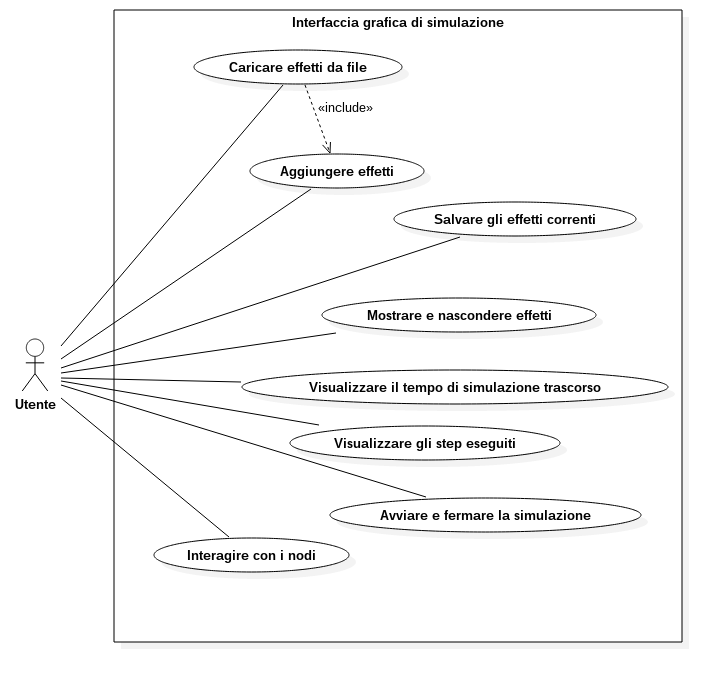
\includegraphics[scale=0.55]{img/useCase}
                    \caption{Requisiti funzionali principali}
                    \label{fig:useCase}
                \end{figure}

        \subsection{Requisiti non funzionali}\label{sub:nonFunzionali}
            I requisiti non funzionali descrivono le proprietà non comportamentali che il sistema deve possedere, come efficienza, affidabilità, sicurezza, performance, ma anche caratteristiche del processo di sviluppo e caratteristiche esterne.

            \subsubsection{JavaFX}\label{subsub:jfx}
                Come specificato nella sezione~\vref{sec:motivi}, il processo di sviluppo deve coinvolgere la libreria JavaFX come framework per la costruzione dell'interfaccia.

            \subsubsection{Performance}\label{subsub:performance}
                L'interfaccia grafica deve quanto più possibile non gravare sulle prestazioni del motore di simulazione; in particolare, poiché JavaFX non è nativamente \engEmph{thread-safe}, è necessario gestire la concorrenza in modo oculato.

            \subsubsection{Supporto Hi-DPI}\label{subsub:hidpi}
                L'interfaccia non deve perdere di usabilità e qualità di rappresentazione su alcun tipo di schermo, indipendentemente dalla risoluzione e dalla densità di pixel.Per fare questo si devono quindi utilizzare quanto più possibile grandezze relative e sfruttare al meglio in tal senso le funzionalità offerte da JavaFX.

            \subsubsection{Serializzazione \engEmph{Human-readable}}
                Deve essere possibile serializzare gli effetti in un formato testo, in modo tale che possa essere facilmente creato e/o modificato manualmente in modo semplice, senza coinvolgere necessariamente l'interfaccia di Alchemist.

    \section{Fonti d'ispirazione}\label{sec:ispirazione}
        Una volta chiariti i requisiti dell'interfaccia, il passo successivo riguarda la progettazione dell'interfaccia.

        Per poter disegnare dei mockup da utilizzare come bozzetti, sono state fatte ricerche in merito alle interfacce grafiche utilizzate da altri simulatori, anche a scopo non strettamente scientifico.

        Infine, si è scelto tra i design moderni più comuni e apprezzati uno da adottare per fornire un aspetto grafico a cui l'utente medio fosse già abituato e che potesse fornire un'esperienza di utilizzo più gradevole.

        \subsection{Simulatori a scopo videoludico}\label{sub:videogame}
            Come già segnalato nelle sezioni precedenti, è importante che l'interfaccia grafica si presenti semplice e immediata anche per l'utente non avanzato. Di conseguenza, si è scelto di analizzare con più attenzione le GUI di simulatori sviluppati a scopo prettamente videoludico, in quanto più orientati all'immediatezza d'uso rispetto ai simulatori di concezione scientifica.

            Tra i videogiochi di simulazione più famosi, è stato interessante analizzare SimCity, il quale all'epoca del lancio fu molto apprezzato~\cite{friedman1995} appunto per il gameplay e l'interfaccia piuttosto innovativi, e i giochi della serie Universe Sandbox del team Giant Army.

            \subsubsection{SimCity}\label{subsub:simcity}
                La celebre serie di videogiochi di simulazione SimCity~\cite{simcity}, ideata da Will Wright tra gli anni `80 e gli anni `90 ispirandosi alla ricerca contenuta nel saggio di architettura \engEmph{A pattern language}~\cite{wiredWright, aPatternLanguage}, sviluppata da Maxis e distribuita da Electronics Arts, è tutt'ora considerata una delle più innovative per quanto riguarda la storia dei videogiochi di simulazione.

                \begin{figure}[htbp]
                    \centering
                    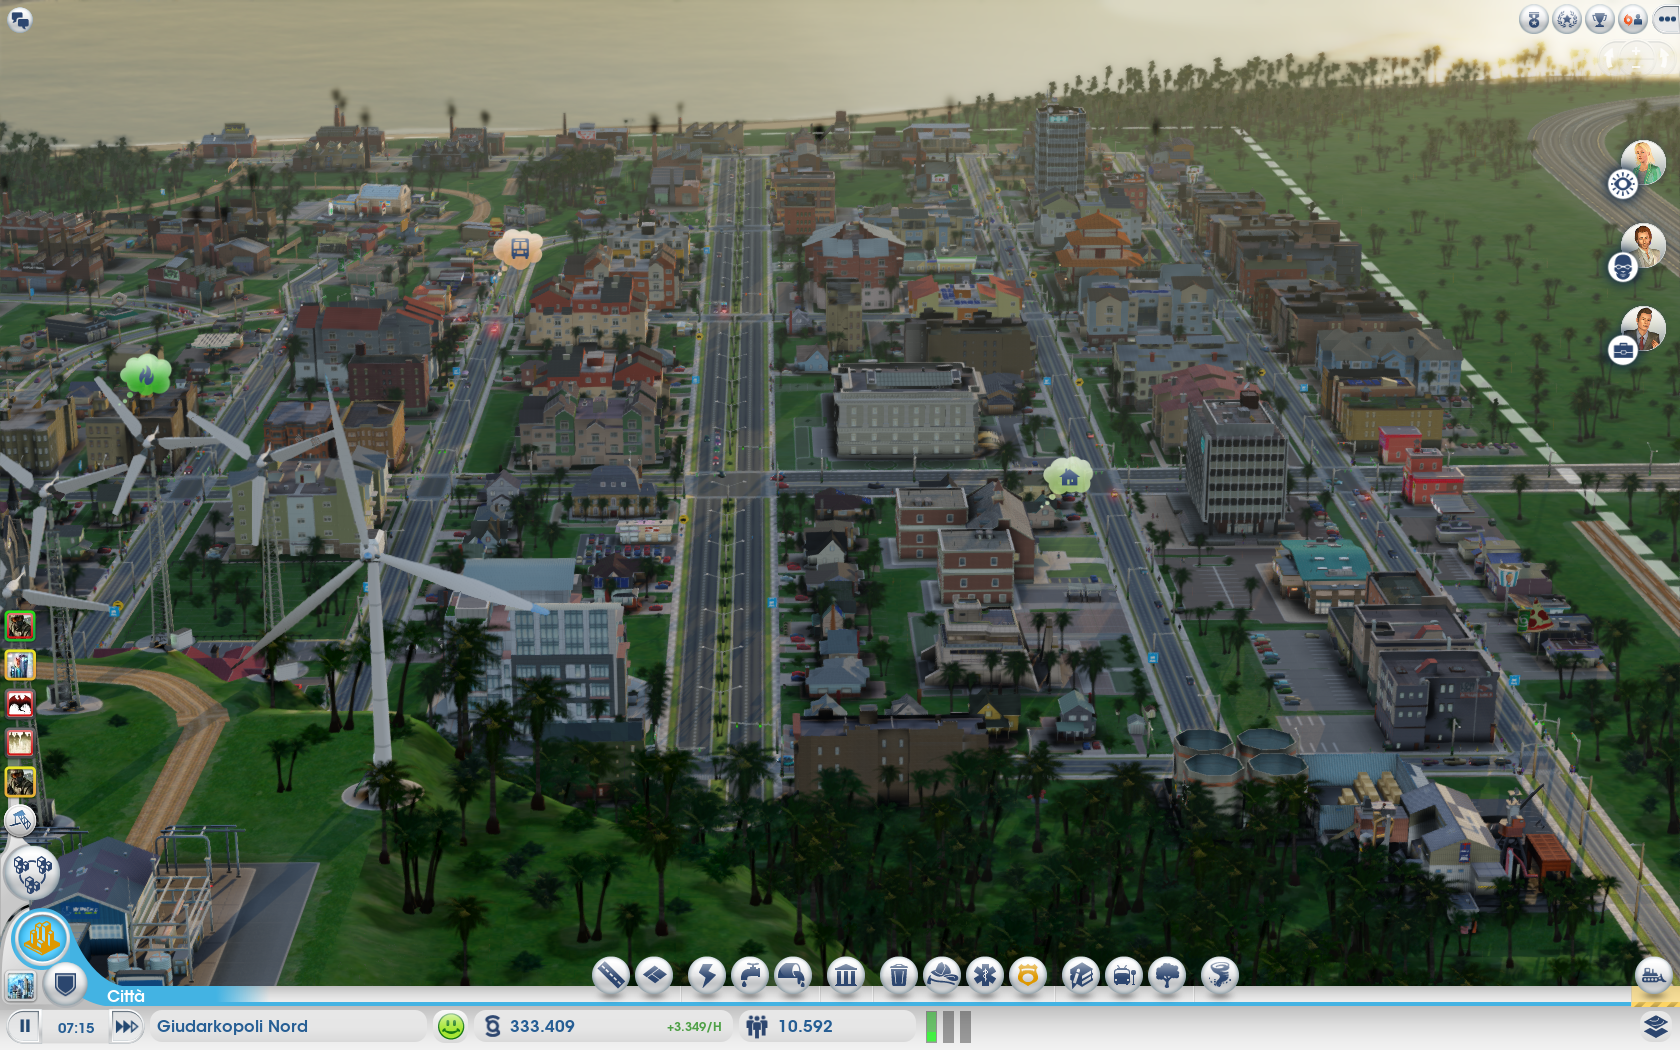
\includegraphics[scale=0.2]{img/SimCity}
                    \caption{SimCity (2013), sviluppato da Maxis e distribuito da EA, tutti i diritti riservati ai ripettivi proprietari}
                    \label{fig:simcity}
                \end{figure}

                % TODO potrebbe essere utile inserire ulteriori dettagli?

            \subsubsection{Universe Sandbox}\label{subsub:universesandbox}
                Altra serie di videogiochi simulativi analizzata è Universe Sandbox.
                Dopo oltre 15 anni di sviluppo~\cite{unisandTechradar}, il primo capitolo~\cite{universeSandboxDixon} è stato rilasciato dallo sviluppatore e artista Dan Dixon nel 2008.
                Il responso positivo lo ha portato a continurare lo sviluppo, tanto da fondare la compagnia Giant Army~\cite{universeSandboxGiantArmy}, che ha rilasciato nel 2015 la seconda iterazione della saga, Universe Sandbox\ap{2}~\cite{universeSandbox2}.

                % TODO approfondire analisi ?

                Per il design dell'interfaccia, è stato proprio il secondo capitolo a fungere da maggior fonte d'ispirazione. Essa va a riprendere la classica interfaccia utilizzata da videogiochi simulativi come il già citato SimCity (\figurename~\ref{fig:simcity}), ma andando a rimuovere buona parte degli ornamenti grafici tipici delle GUI a scopo videoludico, andando a preferire uno stile molto più pulito e semplificato; il sistema di interazione a sviluppo verticale e a popup viene sostituito con uno sviluppo orizzontale di pannelli (definito \emph{Modello multi-paned}~\cite{multipanedmodel}) che vanno a raccogliere tutte le impostazioni e i parametri.

                La simulazione viene rappresentata sullo sfondo, come in SimCity, ma con effetti di trasparenza non presenti nel gioco di EA.

                % TODO approfondire analisi ?

                \begin{figure}[htbp]
                    \centering
                    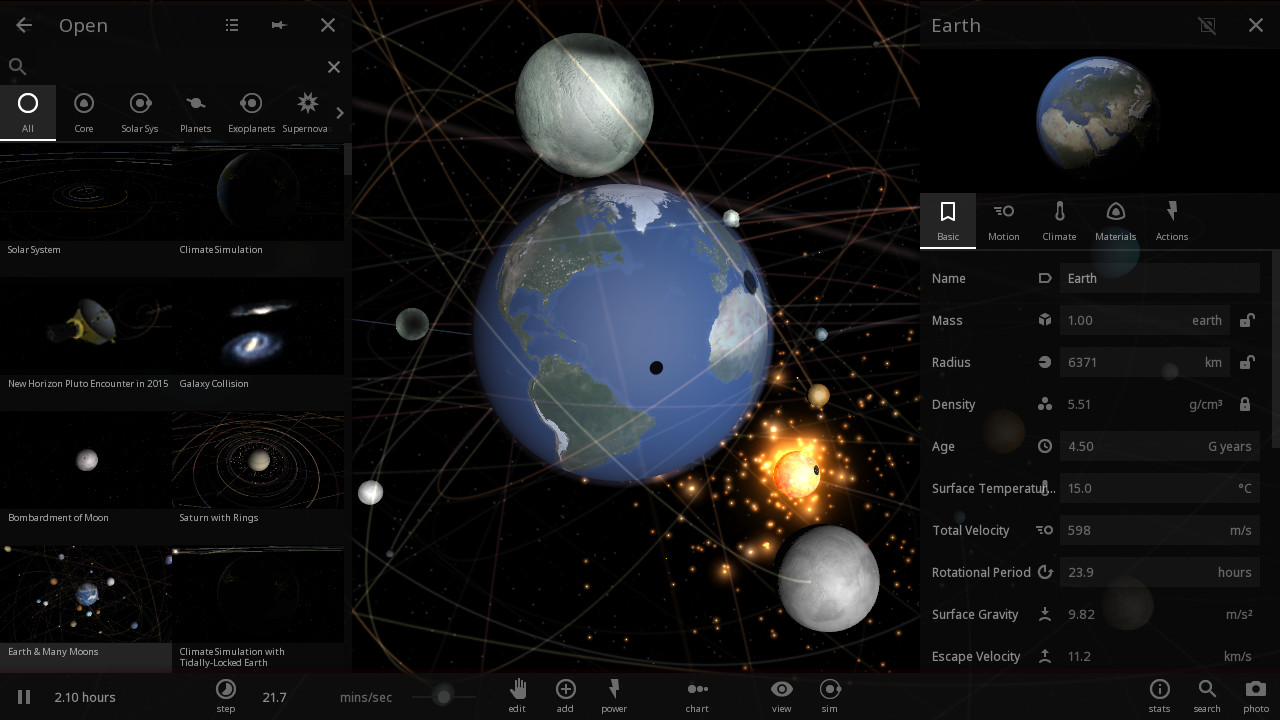
\includegraphics[scale=0.35]{img/universesandboxpanels}
                    \caption{Universe Sandbox\ap{2} (2015), sviluppato e distribuito da Giant Army, tutti i diritti riservati ai ripettivi proprietari}
                    \label{fig:universesandboxpanels}
                \end{figure}

        \subsection{Material Design}\label{sub:material}
            Uno dei maggiori motivi che hanno portato l'interfaccia grafica di Alchemist a necessitare di un rinnovamento è stata l'intenzione di semplificarla all'occhio dell'utente non esperto, fornendo un'esperienza completa e gradevole.
            Era dunque necessario scegliere uno stile grafico familiare, moderno e facilmente adattabile a quella che sarebbe essere la nuova interfaccia che si stava progettando.

            Prendendo come base l'interfaccia di Universe Sandbox illustrata nella sezione~\ref{subsub:universesandbox}, è possibile notare che il design di base sia estremamente ``flat''; si è deciso di valutare i possibili design a cui adeguare la UX che si aveva intenzione di progettare.

            La scelta è infine ricaduta sul Material Design~\cite{material} sviluppato da Google: dal suo annuncio nel giugno del 2014 alla conferenza del Google I/O~\cite{pichai2014google} esso è stato almeno parzialmente adottatto in molte applicazioni web, mobile e desktop, e ben si si presta all'implementazione di un'interfaccia semplice e minimale.

            Si è deciso di utilizzare le icone\footnote{\url{https://material.io/icons/}} e le direttive in merito a dimensioni e palette di colore\footnote{\url{https://material.io/color/}} fornite da Google.

    \section{Design dell'interfaccia}\label{sec:design}
        Una volta chiariti i requisiti e le possibili fonti di ispirazione per la struttura della GUI da realizzare, sono stati disegnati dei mockup che potessero rappresentare una linea guida per l'implementazione concreta dell'interfaccia.

        \begin{figure}[htbp]
            \centering
            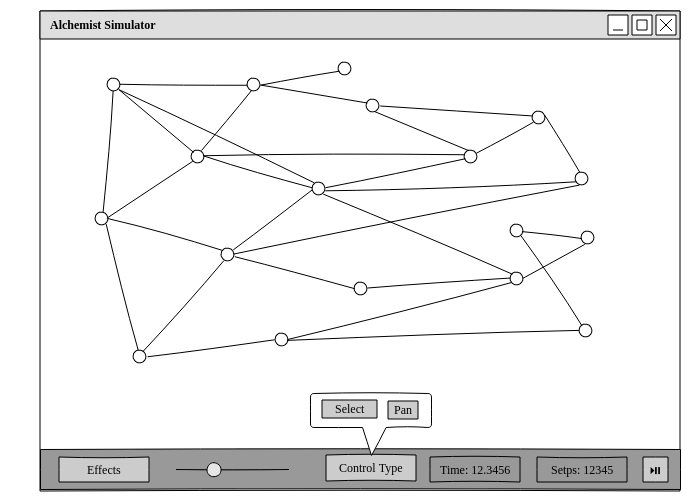
\includegraphics[scale=0.4]{img/withNodes/main_window}
            \caption{Mockup dell'interfaccia principale}
            \label{fig:mock:mainWindow}
        \end{figure}

        Come è possibile vedere dalla \figurename~\vref{fig:mock:mainWindow}, si è scelto di adottare un'interfaccia composta da uno spazio disegnabile centrale, al quale viene sovrapposta nella parte inferiore una barra contenente dei controlli che permettono un'interazione semplice e diretta con le funzionalità di base:

        \begin{description}
          \item [Play/Pausa] Partendo da destra, è presente un bottone che permette di avviare e mettere in pausa la simulazione.

          Esso funge anche da indicatore per lo stato attuale della simulazione: qualora essa venga avviata o fermata da terminale o tramite una scorciatoia da tastiera, l'icona rappresentata sul bottone viene aggiornata per adeguarsi al nuovo stato.

          \item[Avanzamento in termini di tempo e step] Continuando verso sinistra, si trovano spazi dedicati al numero di secondi di simulazione rappresentati e di step effettuati; essi vengono aggiornati durante tutto l'avanzamento del motore di simulazione.

          \item[Gestione del sistema di controllo] Poiché l'interazione tramite mouse deve permettere sia di spostarsi nell'ambiente che selezionare i nodi e interagirvi, è presente un bottone che apre un pannello che permette di scegliere tra spostamento (\engEmph{pan}) e selezione.

          \item[Gestione della velocità] Una barra a scorrimento permette di regolare la velocità di rappresentazione della simulazione.

          \item[Gesione degli effetti] Un bottone sul lato sinistro della barra permette di aprire un pannello sul medesimo lato della finestra per poter controllare gli effetti con i quali rappresentare cosa sta avvenendo nella simulazione.

          Nelle Figure~\vrefrange{fig:mock:groups}{fig:mock:properties} è possibile osservare i diversi livelli del drawer laterale degli effetti.

          \begin{figure}[htbp]
              \centering%
              \subfigure[%
                  Vista dei singoli gruppi di effetti che compongono lo \engEmph{stack}%
                  \label{fig:mock:groups}
              ]{%
                  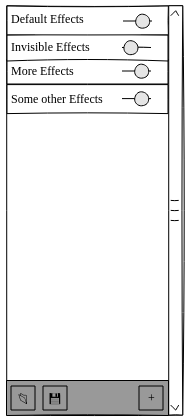
\includegraphics[scale=0.5]{img/cropped/effectgroups_bar_open}
              }%
              \qquad{\LARGE$\Rightarrow$}\qquad
              \subfigure[%
                  Vista dei singoli effetti di un gruppo%
                  \label{fig:mock:effects}%
              ]{%
                  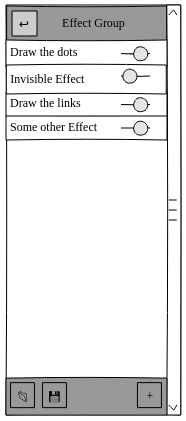
\includegraphics[scale=0.5]{img/cropped/effects_bar_open}
              }%
              \qquad{\LARGE$\Rightarrow$}\qquad
              \subfigure[%
                  Vista delle proprietà di un effetto%
                  \label{fig:mock:properties}%
              ]{%
                  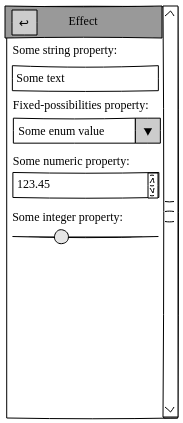
\includegraphics[scale=0.5]{img/cropped/effect_properties_open}
              }
              \caption{Vista del pannello laterale degli effetti nei diversi livelli\label{fig:mock:allEffects}}
          \end{figure}

          % TODO sistema altezza frecce

        \end{description}

    \section{Progettazione}\label{sec:progettazione}
        Terminata la realizzazione dei mockup, il passo successivo riguardava la progettazione della struttura del sistema software.

        \subsection{L'architettura degli effetti}\label{sub:effetti}
            La componente architetturale più complessa da progettare probabilmente è costituita dagli effetti.
            Infatti, concettualmente il nuovo archetipo di effetti (della cui interfaccia è possibile vedere il codice in Appendice~\ref{appendix:effectfx}) rappresenta un oggetto completamente diverso:
            \begin{itemize}
                \item[--] esso non si relaziona più con il singolo nodo, del quale può considerare le proprietà, bensì con l'intero ambiente; in questo modo, l'effetto agisce in blocco su un determinato tipo di entità allo stesso modo, garantendo una migliore uniformità di applicazione.
                \item[--] esso ha un \emph{nome} che lo identifica dalle altre istanze della medesima classe; questo permette all'utente di identificarlo con più semplicità e gestirlo in modo più naturale, soprattutto nel caso si trovi a gestire, attraverso l’interfaccia grafica, una moltitudine di effetti.
                \item[--] esso possiede un campo di \emph{visibilità} individuale, che permette di nasconderlo temporaneamente, aumentando le possibilità di rappresentazione anche per blocchi di effetti predefiniti;
                \item[--] le proprietà peculiari di ciascun effetto sono pensate per implementare il pattern \engEmph{observer}, permettendo di effettuare collegamenti con l'interfaccia in modo trasparente ed ottimizzato, in quanto gestito completamente dal framework di JavaFX.
                \item[--] infine, l'effetto viene serializzato in formato \engEmph{human-readable}, il quale facilita la creazione e la modifica anche al di fuori dell'interfaccia di Alchemist.

                Si è scelto di utilizzare il formato JSON~(JavaScript Object Notation~\cite{json})\footnote{\url{https://www.json.org/index.html}}: esso è un formato di testo per la serializzazione dei dati strutturati, basato sugli oggetti JavaScript, che risulta essere facile da leggere e scrivere per le persone e facile da generare e analizzarne la sintassi per le macchine; è un formato di testo indipendente dal linguaggio di programmazione, ma utilizza convenzioni riconosciute dalla maggior parte dei programmatori di linguaggi.
            \end{itemize}
            
            \begin{figure}[htbp]
                \centering
                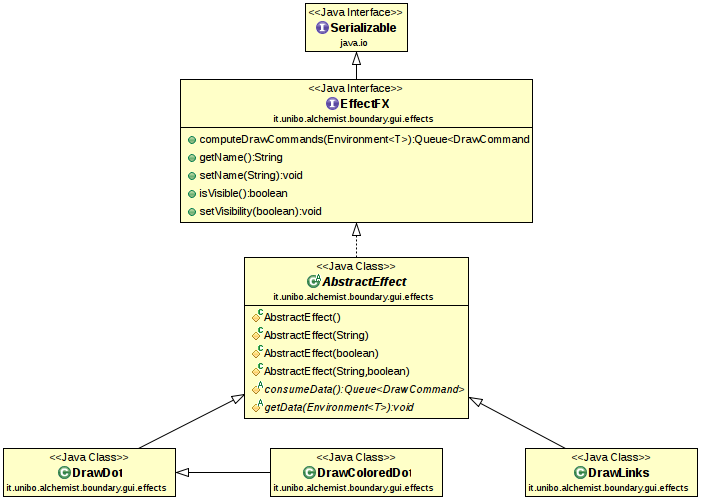
\includegraphics[scale=0.55]{img/EffectFXUMLsimple}
                \caption{Diagramma UML delle classi che modellano la nuova struttura di effetti; maggiori dettagli in Appendice~\ref{appendix:effectfx}} % TODO verifica e sistema riferimento
                \label{fig:effectFX}
            \end{figure}

            Come rappresentato graficamente nel diagramma UML in \figurename~\vref{fig:effectFX}, un effetto viene concretizzato secondo il pattern \engEmph{template method}: la struttura di funzionamento di base viene parzialmente definita da una classe astratta che implementa il metodo principale dell'interfaccia effetto, \texttt{computeDrawCommands()}, come metodo template, il quale chiama i due metodi astratti \texttt{getData()} e \texttt{consumeData()} per adempiere al proprio compito.
            La suddivisione permette a ciascun effetto concreto di separare le procedure che coinvolgono l'interrogazione del modello da quelle che portano alla costruzione della coda di comandi per effettuare la rappresentazione grafica.

        % TODO gruppi di effetti

        \subsection{La barra inferiore}\label{sub:barra}
        \subsection{La struttura a drawer}\label{sub:drawer}
            % \subsubsection{I gruppi di effetti e l'interfaccia \texttt{EffectGroup}}\label{subsub:effectGroup}
            % \subsubsection{I singoli effetti e l'interfaccia \texttt{EffectFX}}\label{subsub:effectFX}
            % \subsubsection{Caricamento, salvataggio e modifica di gruppi di effetti}\label{subsub:serializzazione}
    \section{Dettagli implementativi}\label{sec:dettagli}
        % \subsection{Librerie utilizzate}\label{sub:lib}
        % \subsection{Gestione della concorrenza}\label{sub:concorrenza}

    %% Direttive TeXworks:
% !TeX root = ../../maltoni_niccolo_tesi.tex
% !TEX encoding = UTF-8 Unicode
% !TEX program = arara
% !TEX TS-program = arara
% !TeX spellcheck = it-IT

%% Direttive Arara:
% arara: pdflatex: { shell: yes, synctex: yes, action: batchmode, options: "-halt-on-error -file-line-error-style" }
% arara: frontespizio
% arara: biber
% arara: pdflatex: { shell: yes, synctex: yes, action: batchmode, options: "-halt-on-error -file-line-error-style" }
% arara: pdflatex: { shell: yes, synctex: yes, action: nonstopmode, options: "-halt-on-error -file-line-error-style" }

\chapter{Conclusioni}\label{ch:conclusioni}
    \section{Risultati}\label{sec:risultati}
        L'obiettivo di questa tesi era quello di realizzare un'interfaccia grafica per l'ambiente di simulazione di Alchemist che sostituisse la precedente e si andasse ad integrare con i recenti contributi dati ad altre sezioni della GUI del software, andando a fornire una esperienza utente più semplice e gradevole anche per i meno esperti.

        L'interfaccia, realizzata con la libreria JavaFX, ha comportato un restyling completo a livello estetico e una reimplementazione di numerose parti del codice.
        Al termine del lavoro illustrato in questa tesi, essa risulta essere in grado di caricare una simulazione, rappresentarla a schermo attraverso effetti importabili ed esportabili per mezzo di file JSON e controllarne il flusso d'esecuzione; l'impatto sulle performance di simulazione rispetto a un'esecuzione \engEmph{headless} è accettabile e nei margini di quanto previsto.

        Di seguito è possibile vedere alcuni screenshot della GUI con una simulazione in esecuzione (\Crefrange{fig:simWithNodes}{fig:simWithDnD}).

        \begin{figure}[htbp]
            \centering
            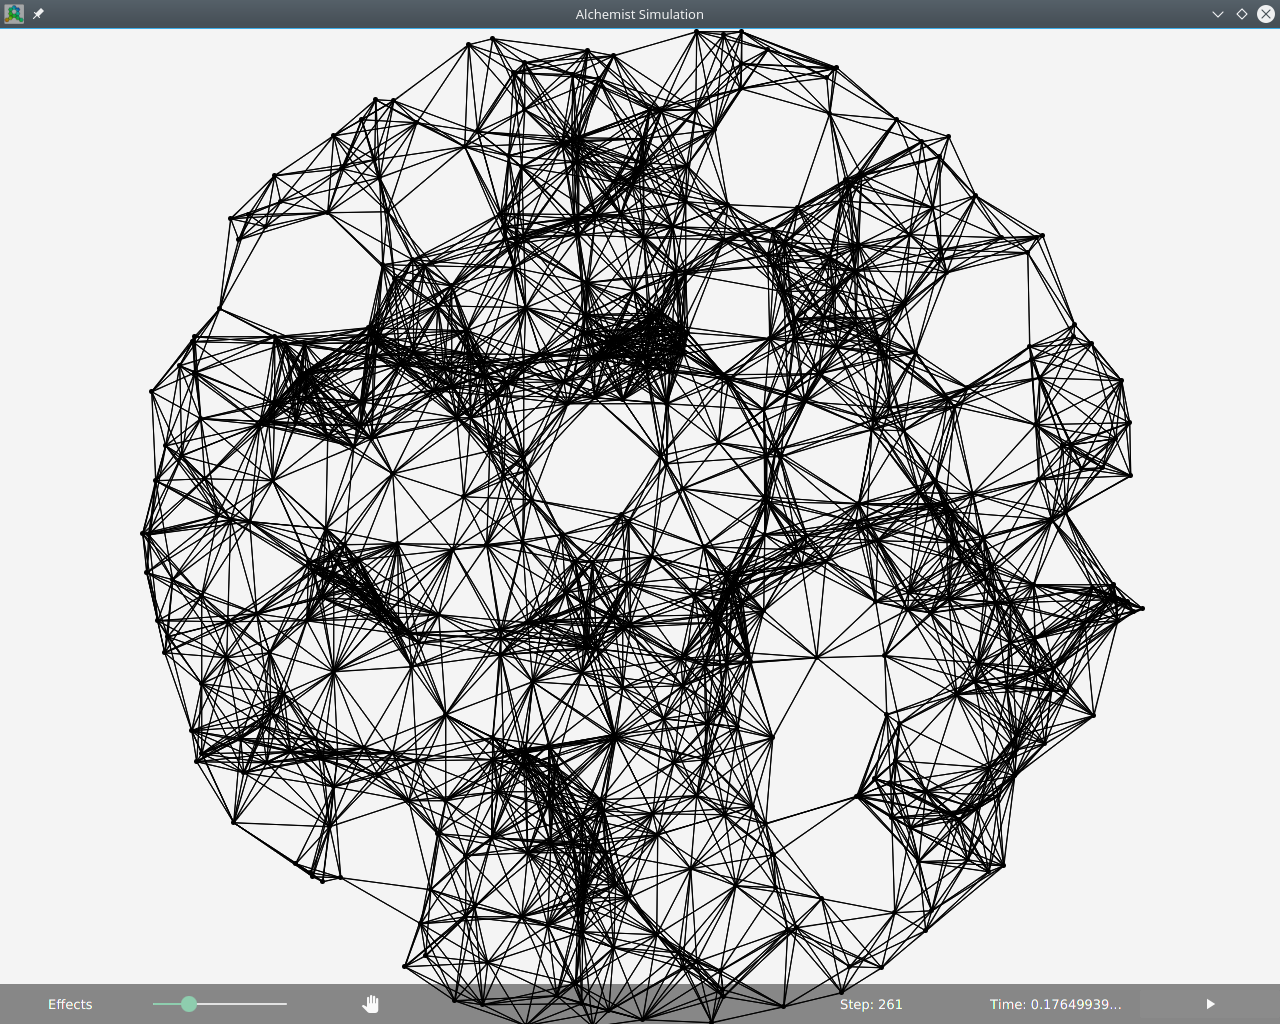
\includegraphics[scale=0.45]{img/withNodes/simWithNodes}
            \caption{Simulazione in corso di esecuzione}
            \label{fig:simWithNodes}
        \end{figure}

        \begin{figure}[htbp]
            \centering
            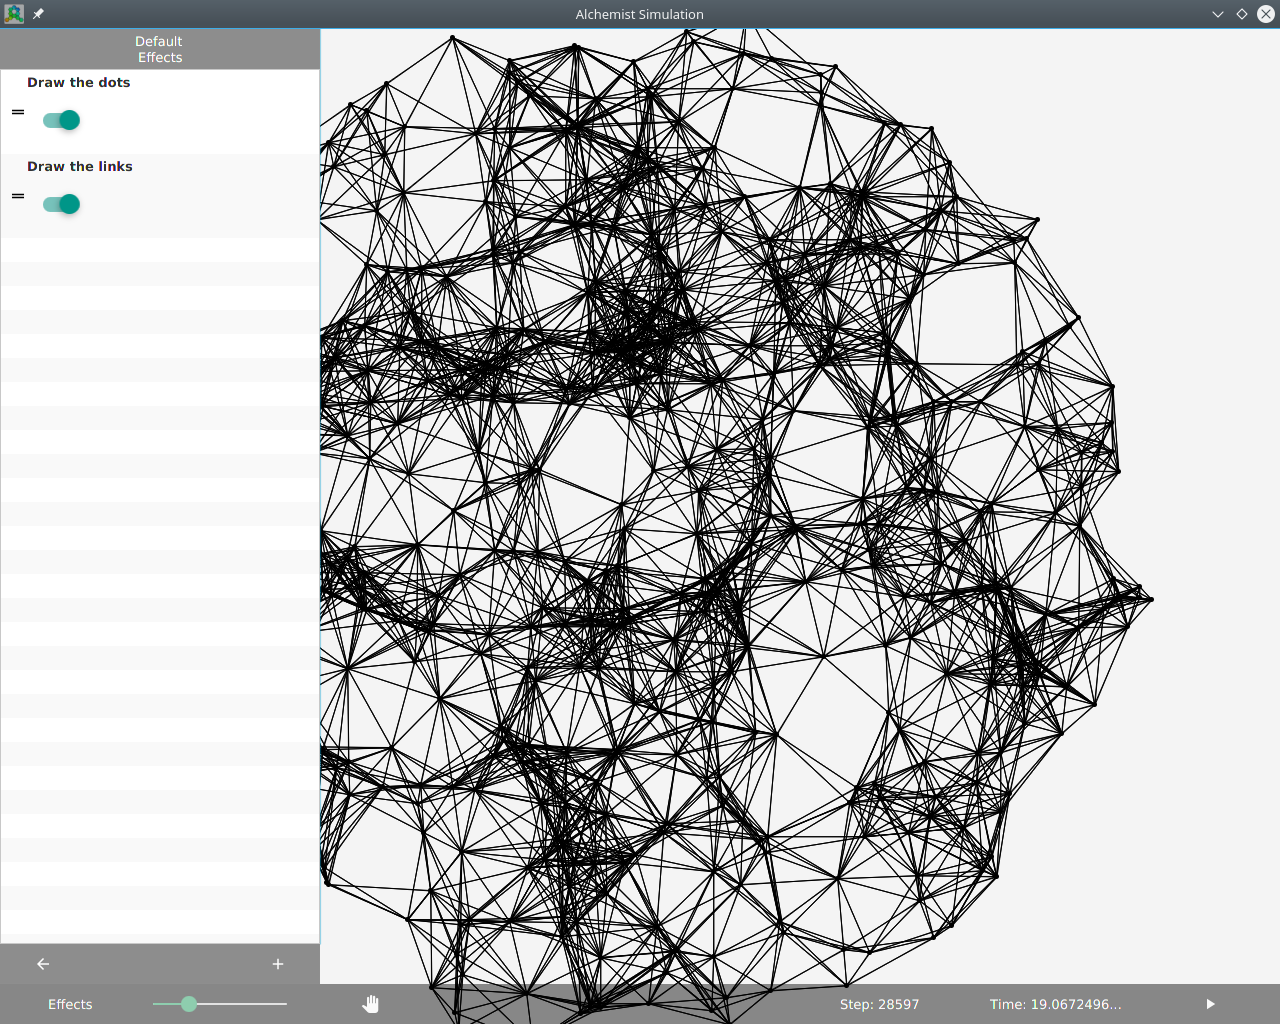
\includegraphics[scale=0.45]{img/withNodes/simWithEff}
            \caption{Drawer laterale degli effetti aperto}
            \label{fig:simWithEff}
        \end{figure}

        \begin{figure}[htbp]
            \centering
            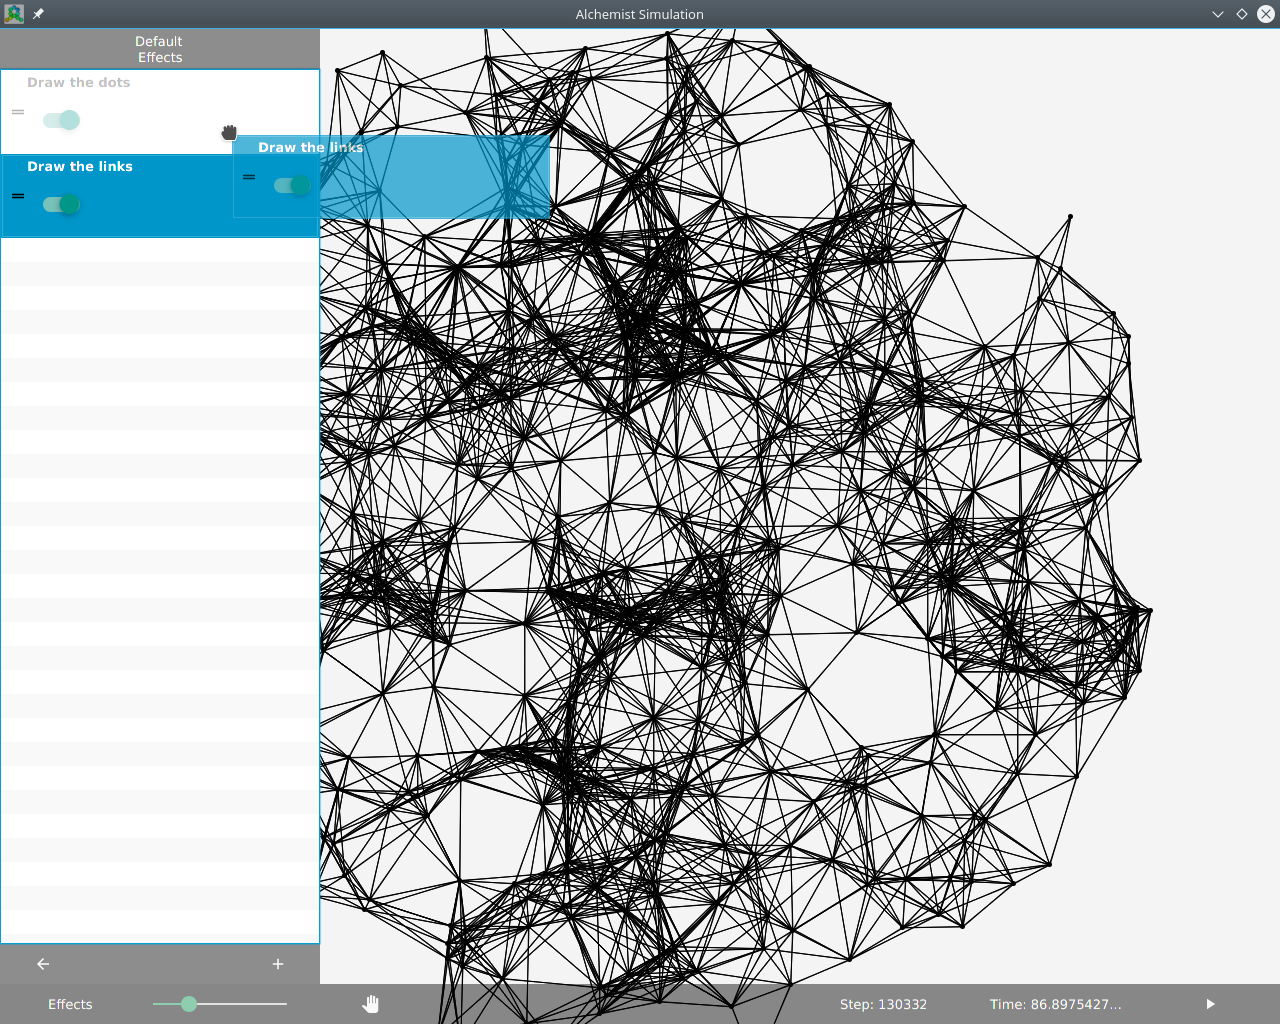
\includegraphics[scale=0.45]{img/withNodes/simWithDnD}
            \caption{Gestione \engEmph{Drag'n'Drop} degli effetti}
            \label{fig:simWithDnD}
        \end{figure}

        Nonostante il lavoro svolto sia funzionante, la mole di lavoro necessario non ha permesso di soddisfare tutti i requisiti e pertanto non può ancora sostituire completamente l'interfaccia classica. Nel paragrafo successivo sono illustrati i lavori futuri che possono essere apportati per rendere la GUI utilizzabile nel ramo stabile.

    \section{Lavori futuri}\label{sec:futuro}
        \textbf{\texttt{[...]}}


    % %% Direttive TeXworks:
% !TeX root = ../maltoni_niccolo_tesi.tex
% !TEX encoding = UTF-8 Unicode
% !TEX program = arara
% !TEX TS-program = arara
% !TeX spellcheck = it-IT

\appendix
\begin{appendices}
    \chapter{Simulazione di prova}\label{app:test}
        \section{YAML della simulazione}\label{app:yaml}
            \lstinputlisting[language=yaml]{data/simulation.yml}
            \clearpage

        \section{JSON degli effetti}\label{app:json}
            \lstinputlisting[language=json]{data/effects.json}
            \clearpage

        \section{AES degli effetti}\label{app:aes}
            \lstinputlisting[language=json]{data/effects.aes}
\end{appendices}
    % \chapter{Codice relativo all'interfaccia classica}\label{app:old}
        % \section{L'interfaccia \texttt{Effect}}\label{app:effect}
            % TODO codice

    % \chapter{Codice relativo al contributo}\label{app:new}
        % \section{L'interfaccia \texttt{EffectFX}}\label{app:effectfx}
            % TODO codice
        % \chapter{L'interfaccia \texttt{EffectFX}}\label{app:effectfx}
            % TODO UML

        % \section{L'interfaccia \texttt{EffectGroup}}\label{app:effectgroup}
            % TODO codice

        %\section{Implementazioni di \texttt{EffectFX} e Proprietà serializzabili}\label{app:effectsAndProps}
            % TODO codice
        % \chapter{Implementazioni di \texttt{EffectFX} e Proprietà serializzabili}\label{app:effectsAndProps}
            % TODO UML
            % \begin{figure}[htbp]
                % \centering
                % 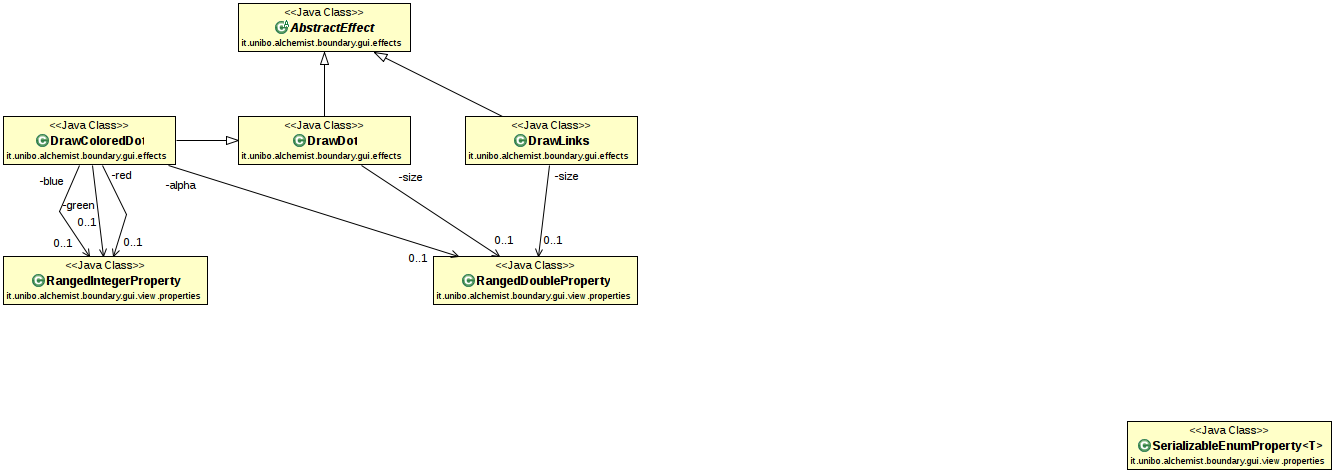
\includegraphics[scale=0.7]{img/EffectAndPropertiesUML}
                % \caption{Il diagramma UML delle classi mostra le relazioni tra gli effetti implementati e le proprietà custom utilizzate}
            % \end{figure}


    \backmatter
    %% Direttive TeXworks:
% !TeX root = ../maltoni_niccolo_tesi.tex
% !TEX encoding = UTF-8 Unicode
% !TEX program = arara
% !TEX TS-program = arara
% !TeX spellcheck = it-IT

%% Direttive Arara:
% arara: pdflatex: { shell: yes, synctex: yes, action: batchmode, options: "-halt-on-error -file-line-error-style" }
% arara: frontespizio
% arara: bibtex
% arara: pdflatex: { shell: yes, synctex: yes, action: batchmode, options: "-halt-on-error -file-line-error-style" }
% arara: pdflatex: { shell: yes, synctex: yes, action: nonstopmode, options: "-halt-on-error -file-line-error-style" }

% \chapter*{Bibliografia}
\addcontentsline{toc}{chapter}{Bibliografia}
\bibliography{biblio}
\nocite{mysite}
\bibliographystyle{abbrv}
% Possibili stili:
% - plain (ordine alfabetico contrassegnato da numeri),
% - unsrt (ordine di citazione contrassegnato da numeri),
% - alpha (opere contrassegnate da etichette formate a partire dal nome dell’autore e dall’anno di pubblicazione),
% - abbrv (come plain, ma i nomi di battesimo, i nome dei mesi e dei giornali sono abbreviati)

    % \listoffigures
    % \listoftables
    % %% Direttive TeXworks:
% !TeX root = ../../maltoni_niccolo_tesi.tex
% !TEX encoding = UTF-8 Unicode
% !TEX program = arara
% !TEX TS-program = arara
% !TeX spellcheck = it-IT

\chapter*{Ringraziamenti}
% \addcontentsline{toc}{chapter}{Ringraziamenti}
Un sincero ringraziamento va a tutti coloro che mi hanno aiutato in vario modo a raggiungere questo traguardo.
Ringrazio il professor Mirko Viroli e il professor Danilo Pianini per l'aiuto datomi nella realizzazione di questo progetto, sia durante l'attività sperimentale che per la stesura dell'elaborato finale.
Ringrazio anche gli amici che ho avuto vicino in questi mesi, ma soprattutto un particolare grazie ai miei familiari che mi sostengono da sempre.

\end{document}
